\newpage
\fontsize{22pt}{16pt}\selectfont
\begin{center}
    {\bfseries Lời mở đầu}
\end{center}
\fontsize{13pt}{16pt}\selectfont
\bigskip

Với sự phát triển khoa học kỹ thuật trên toàn cầu, nguồn dữ liệu thông tin khảo sát của mỗi một doanh nghiệp, tập đoàn ngày càng nhiều và tăng trưởng theo cấp số nhân. Với nhu cầu tiếp nhận, phân tích và xử lý dữ liệu dưới góc nhìn đa chiều và tổng hợp hiện nay, việc thống kê dòng dữ liệu là vô cùng cần thiết, từ đó khái niệm kho dữ liệu ra đời nhằm đảm lưu trữ đầy đủ dữ liệu cho bước phân tích tiếp theo và nâng cao tốc độ của các kết quả trả về của hệ thống. Cùng với Data Warehouse thì Dashboard cũng là một công cụ không thể thiếu trong các hoạt động kinh doanh, quản lý của tổ chức. Nhờ có Dashboard mà nhà quản trị có cái nhìn tổng quan, chi tiết và cụ thể cho hướng đi của doanh nghiệp.\\

Thế giới có nhịp độ nhanh ngày nay đã ảnh hưởng không nhỏ đến sức khỏe của chúng ta. Điều rất quan trọng là phải tiêu thụ thực phẩm lành mạnh và có một chế độ ăn uống cân bằng, tập luyện để giữ cho chúng ta khỏe mạnh về thể chất và tinh thần.\\

Dựa vào nhu cầu đó nhóm 9 quyết định chọn chủ đề HEALTH CARE để tìm
hiểu và báo cáo về các khảo sát sức khỏe của mọi người dựa vào các nhân tố ảnh hưởng đến sức khỏe như tuổi tác, các bệnh nền từ bộ dữ liệu của hệ thống giám sát yếu tố rủi ro hành vi BRFSS.\\

Chúng em xin gửi lời cảm ơn đến thầy ThS. Nguyễn Danh Tú đã hướng dẫn và đưa ra những góp ý cho nhóm hoàn thành đề tài.

\begin{minipage}{0.5\textwidth}
\end{minipage}
\hspace{0.5\textwidth}
\begin{minipage}{0.5\textwidth}
	\noindent\begin{center}
		\vspace{1cm}
		\textit{Hà Nội,ngày 26 tháng 7 năm 2022} \\
		Thay mặt nhóm báo cáo\\ \vspace{1cm}
		\textbf{Nhóm 9}\\
	\end{center}	
\end{minipage}

\bigskip

\newpage
%%%%%%%%%%%%%%
\newpage
\fontsize{22pt}{16pt}\selectfont
\begin{center}
    {\bfseries Đánh giá các thành viên}
\end{center}
\fontsize{13pt}{16pt}\selectfont
\bigskip

\subsection*{Các thành viên trong nhóm}
\begin{enumerate}
    \item  Nguyễn Thị Duyên - 20195866
    \item  Phạm Thị Hoa - 20195874
    \item  Trần Thị Hồng -20195880
    \item Phạm Thu Trang -20195931
    \item Trần Thị Hồng Vân - 20195941
\end{enumerate}

\subsection*{Đánh giá: }
\textbf{Bảng đánh giá các thành viên trong nhóm}
\begin{center}
            \begin{figure}[!h]
                \centering
                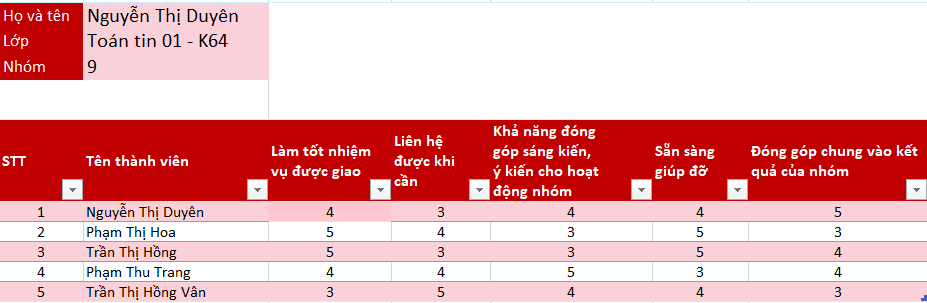
\includegraphics[scale = 0.8]{contents/Bảng đánh giá thành viên.PNG}
              \caption{Bảng đánh giá thành viên}
            \end{figure}
\end{center}
Trong quá trình hoạt động, các thành viên trong nhóm đều có tinh thần làm
việc tốt, hoàn thành tốt nhiệm vụ được giao và đều đóng góp vào trong kết quả
của nhóm, từ khâu chọn dữ liệu đến việc phân tích, xử lý dữ liệu và vẽ Dashboard.
Với tinh thần làm việc nhóm tốt, mọi người đã hoàn thành công việc đúng hạn và báo cáo Dưới đây là công sức của cả 5 thành viên đã cố gắng trong 16 tuần vừa qua.

\bigskip
\newpage
%%%%%%%%%%%%%%%%%%%%%%%%%%%%%%%%%%
\fontsize{22pt}{16pt}\selectfont
\begin{center}
    {\bfseries Tự đánh giá báo cáo nhóm}
\end{center}
\fontsize{13pt}{16pt}\selectfont
\bigskip
\begin{enumerate}
    \item \textbf{Mục tiêu và nội dung của báo cáo}
\begin{enumerate}
    \item \textbf{Mục tiêu:}\\
Sau khi hoàn thành báo cáo, chúng em sẽ nắm rõ được những khái niệm cơ bản về phân tích dữ liệu; hiểu được quy trình phân tích dữ liệu và triển khai vào công việc thực tiễn; Làm chủ được các công cụ trực quan hóa dữ liệu như Excel, Power BI và Hệ quản trị cơ sở dữ liệu để lựa chọn giải pháp tốt nhất trong thực tế.
\item \textbf{Nội dung của bài Báo cáo:}
\begin{itemize}[label=$-$]
    \item Tổng quan về Data Warehouse.
    \item Tổng quan về Heathycare
    \item Phân tích nghiệp vụ.
    \item Đưa ra requirement khi xây dựng kho dữ liệu.
    \item Kiến trúc Data Warehouse
    \item  Sơ đồ quá trình ETL và các nội dung ETL bằng Power Query và SQL
    \item Xử lý dữ liệu và vẽ sơ đồ dữ liệu OLTP
    \item  Sơ đồ các chiều dữ liệu
    \item Đưa dữ liệu từ cơ sở dữ liệu vào công cụ phân tích Power BI và OLAP hoá.
    \item Vẽ sơ đồ dữ liệu OLAP
    \item  Vẽ các dashboard theo chủ đề
    \item Phân tích các dashboard.
\end{itemize}
\end{enumerate}
\item \textbf{Kết quả đạt được:}
\begin{itemize}[label=$-$]
    \item  Hiểu được những kiến thức nền tảng cơ bản về Kho dữ liệu, Kinh doanh
thông minh, phân tích dữ liệu và phân tích kinh doanh. Bên cạnh đó xây dựng được kiến trúc của kho dữ liệu.
    \item  Nắm rõ được quy trình phân tích dữ liệu.
    \item Phân tích và thiết kế được các mô hình của hệ thống mới.
    \item Làm chủ được một số công cụ trực quan hóa dữ liệu như Excel, Power BI.
    \item Khảo sát và làm việc trên bộ dữ liệu thực tế
    \item Xây dựng được kiến trúc kho dữ liệu ứng với bài toán thực tế của nhóm.
    \item ETL dữ liệu trên các công cụ Excel, Power Query
    \item Vẽ được sơ đồ OLTP
    \item Xác định được các chiều phân tích của bài toán
    \item  Xây dựng được mô hình dữ liệu OLAP và đưa vào công cụ trực quan hóa Power BI.
    \item Xây dựng được các dashboard phân tích và tổng quan.
    \item Phân tích được các dashboard theo các chiều dữ liệu đã xác định.
    \item Tiếp cận đến các công cụ mới để phân tích dữ liệu và xây dựng DW
như SQL Server Analysis Service...
\end{itemize}
\item \textbf{Nội dung chưa làm được:}
\begin{itemize}[label=$-$]
    \item Chưa xử lý thành thạo bộ dữ liệu kích thước lớn, và còn thiếu dữ liệu ban đầu.
    \item Sử dụng công cụ trực quan hóa Power BI chưa được chuyên nghiệp, các Dashboard chưa phân tích sâu các chiều dữ liệu.
\end{itemize}
\item \textbf{Bài học thu được:}
\begin{itemize}[label=$-$]
    \item Việc xây dựng kho dữ liệu là vô cùng cần thiết cho mục đích phân tích dữ liệu.
    \item Dữ liệu trong thực tế không phải lúc nào cũng được chuẩn hóa theo một
quy tắc và không dữ liệu nào là hoàn hảo. Vì vậy luôn cần phải xử lý
trước khi đưa vào hệ thống.
\item Quá trình ETL dữ liệu rất quan trọng và tốn nhiều thời gian nên đòi
hỏi cần phải tập trung quan tâm thực hiện. Cần nghiên cứu bộ dữ liệu
một cách tỉ mỉ để xử lý dữ liệu một cách đúng đắn để tránh xảy ra sai
sót và mất dữ liệu
\item Dữ liệu có kích thước lớn gây ảnh hưởng đến thời gian chạy của máy
tính, cần chọn máy có cấu hình phù hợp cho việc xử lý và phân tích.
Và có thể chia nhỏ các file để dễ dàng thực hiện.
\item  Kiến thức nghiệp vụ của mỗi quy trình là vô cùng quan trọng, vì khi
hiểu được nghiệp vụ chúng ta mới có thể xây dựng được một hệ thống
BI đúng và hiệu quả. Vì vậy, đầu tiên cần phải khảo sát thật kỹ nghiệp
vụ của từng quy trình hoạt động.
\item  Mô hình dữ liệu đa chiều giúp phân tích dữ liệu trên nhiều góc nhìn
khác nhau, và có thể phân cấp.
\item Các dashboard nên được xây dựng theo hướng chủ đề, phải đảm bảo
tính logic và thẩm mỹ.
\end{itemize}
   
%\end{enumerate}
\end{enumerate}
\newpage
%%%%%%%%%%%%%%%%%%%%%%%%%%%%%%%%%%
%\tableofcontents
\newpage
\listoffigures
%\newpage
%\listoftables

